% !TEX root = ./../main.tex
\chapter{MD tools, parallelization and hardware acceleration}
%Manuale GROMACS 3.17.5 PP/PME ranks

%http://www.gromacs.org

\section{GROMACS package}
The \ac{MD} tool and the main analysis tool used in this thesis work is the \href{http://www.gromacs.org}{\gromacs}\cite{gromacsManual} package. It is compatible with both atomistic and \ac{CG} \acp{FF} and support a variety of options and parameters such as different thermostat and barostat algorithms, different methods to treat the electrostatic interaction such as the \ac{ESM} and the \ac{PME} method, different integrators, cut--off schemes and so on. For what concern the trajectory analysis it holds a comprehensive framework for obtaining different quantities. Moreover it supports different kind of parallelization that is it has the compatibility with both multi--core single processor (home PC) and multi--core multi--processor (cluster) architectures with the support of both MPI and OpenMP libraries and the support of different hardware accelerated frameworks such as CUDA\textsuperscript{®}, OpenCL and OpenACC.  

\subsection{Parallelization}
Parallelization refers to the possibility of running a program, in this case an \ac{MD} simulation, in concurrency with the use of more then one CPUs or more then one cores per CPUs or both. The efficiency of a parallelization scheme is mainly determined by how much information each core and/or CPU has to exchange with the others, the least the better. The reason is that the libraries (MPI and OpenMP) needed for the exchange of the information are not fast as the cores are. Hence when the waiting time for the exchange of information becomes higher than the total time spent in executing the parallel code the program has reach its scaling limit, that is, no more CPUs or cores has to be used.

For what concern an \ac{MD} simulation there exists indeed one main kind of parallelization scheme: the domain decompositions. Domain decomposition exploits the local character of most of the interactions used in common \acp{FF}. The simulation box is dived into cells, each of which is assigned to a cores such that it store only a portion of the whole system: the particles which lie in that region and forces between them and the atom positions and forces from neighboring regions owned by other cores. In order to minimize the communication between different cores each cells has to minimize its surface respect to the volume, so it is important to use cells that are as cubic as possible. Indeed, in any case, if the cells are not too small, the particle update can be carried out every time the neighbor list is updated, this also contribute to reduce the number of communication. A common choice is to use cell greater than two times the cut-off radius. The scaling limit with the domain decomposition is reach when the cells are too small that few particles lied in each cell; for \gromacs it means $\sim 100 \div 200$~atoms/core.

\subsection{PP and PME nodes}
When using the \ac{PME} method for the electrostatic interaction a special parallelization is needed in order to speed up the simulation. The reason is related to the fact that the \ac{PME} method intrinsically need to know all the particle positions in the whole simulation box; in a domain decomposition scheme it results in a massive use of the so called \textit{all--to--all} communications, i.e. all cores have to communicate to each other. Hence this leads to a loss of computational performance. In order to minimize the all--to--all communications \gromacs implement the possibility to assign a subset of the cores exclusively to the calculation of the energy contribution of the electrostatic interaction using the \ac{PME} method while the rest of the work is assigned to the remaining cores, called the \ac{PP} cores. In figure~(\ref{fig:PMENodes}) a schematic view of the all--to--all communications in a comparison between \ac{PP}/\ac{PME} in the same cores and the use of the separate \ac{PME} cores is shown. As one can see the all--to--all communications (red arrow) are smaller for the separate \acs{PME} scheme then that for \ac{PP}/\ac{PME} scheme.
\begin{figure}[h!t]
	\centering
	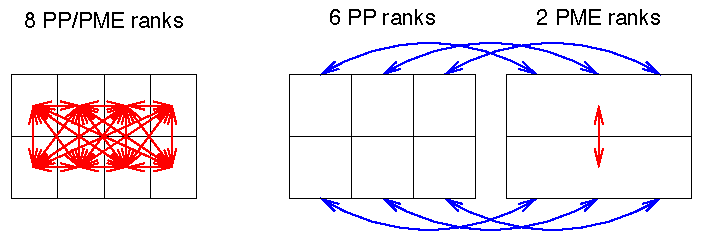
\includegraphics[width=0.8\textwidth]{./img/PMENodes}
	\caption{Left: example of the use of $8$ cores for both \acs{PP} and \acs{PME}. Right: same but $2$ cores are used only for \acs{PME} and the other for the \acs{PP} contribution. Red arrows represent the all--to--all communications while the blu arrows are the communications between one \acs{PP} core and one \acs{PME} core. Taken from \cite{gromacsManual}.}
	\label{fig:PMENodes}
\end{figure} 

To optimize the load in the \ac{PME} cores a domain decomposition is still used but with a $2$D or a ``pencil'' scheme. This because the \ac{FFT} method is very inefficient if parallelized with too many cores due to the all--to--all communications, thus the domain decomposition acts on $xy$--plane while the $z$ axis is assigned to a specific core; pencil refers to the shape of the domain at high parallelization. Moreover the number of domains  along the $x$ axes have to be equal to the number of domains in the \ac{PP} decomposition and eventually a $1$D scheme can be used along the $y$ axis only if the \ac{PP} decomposition has one domain along $x$ axis. To avoid superfluous communication of coordinates and forces between the \ac{PP} and \ac{PME} cores, the number of cells along the $x$ axis should ideally be the same or a multiple of the number of \ac{PME} cores. Most of this issues are taken into account approximately automatically by \gromacs at the begging of the simulation.

\subsection{Hardware acceleration}


\section{PLUMED package}

\section{Simulation parameters}


\begin{table}[h!t]
	\centering\footnotesize
	\begin{tabular}{lcccc}
		\toprule
		Input parameter & Eq. \acs{PME} & Run \acs{PME} & Eq. \acs{PME}\&\acs{PW} & Run \acs{PME}\&\acs{PW} \\ \toprule
		Time step [fs]		&	$10$ & $20$ & $5$ & $20$ \\ \midrule
		cut--off scheme		& Verlet & Verlet & Verlet & Verlet \\ \midrule
		VbT$^a$ [J/(mol ps)]& $5$ & $5$ & $5$ & $5$ \\ \midrule
		Coulomb Type		& \acs{PME}	& \acs{PME}	& \acs{PME} & \acs{PME} \\ \midrule
		$r$ Coulomb	[nm]	& $1.2$ & $1.2$ & $1.2$ & $1.2$ \\ \midrule
		$\varepsilon_r$		& $15$ & $15$ & $2.5$ & $2.5$ \\ \midrule
		\acs{FFT} grid [nm]	& $0.12$ & $0.12$ & $0.12$ & $0.12$ \\ \midrule
	    \acs{PME} order		& $4$ & $4$ & $4$ & $4$ \\ \midrule
		VdW$^b$ type		& cut--off & cut--off & cut--off & cut--off \\ \midrule
		$r$ VdW [nm]		& $1.2$ & $1.2$ & $1.2$ & $1.2$ \\ \midrule
		$T$ coupling		& $v$--rescale & $v$--rescale & $v$--rescale & $v$--rescale \\ \midrule
		$T$ [K]				& $310$ & $310$ & $310$ & $310$  \\ \midrule
		$\tau_T$ [ps]		& $2.0$ & $2.0$ & $2.0$ & $2.0$ \\ \midrule
		$p$ coupling		& Berendsen & Parrinello--Rahman & Berendsen & Parrinello--Rahman \\ \midrule
		$p$ type			& semiisotropic & semiisotropic & semiisotropic & semiisotropic \\ \midrule
		$p$ [bar]			& $1.0$,$1.0$ & $1.0$,$1.0$ & $1.0$,$1.0$ & $1.0$,$1.0$ \\ \midrule
		$\tau_p$ [ps]		& $4.0$,$4.0$ & $12.0$,$12.0$ & $4.0$,$4.0$ & $12.0$,$12.0$ \\ \midrule
		$K^c$ [bar$^{-1}$]	& $4.5\cdot 10^{-5}$ & $3.0\cdot 10^{-4}$ & $4.5\cdot 10^{-5}$ & $3.0\cdot 10^{-4}$ \\ \midrule
		$v$ random			& yes ($310$~K) & no & yes ($310$~K) & no \\ \bottomrule 
	\end{tabular}
	\caption{Summary of the main input parameters used in my \acs{MD} runs. $^a$ Verlet--buffer--tollerance. $^b$ Van der Waals. $^c$ System compressibility.}
	\label{tab:inputParam}
\end{table}
